\chapter{Deep Network}
\section{Deep learning}
Deep learning is a part of machine learning. It includes the methods based on learning data representation by allowing the computation on the models that are composed of multiple layers. Each layer extracts the representaion of the input data from the previous layer and computes a new presentation as the input for the next layer. In the hierachy of a model, the higher layers of representation enlarge aspects of the input that is important for discrimination and suppress irrelevant variations. Each level of representations is corresponding to the different level of abstraction. Deep learning methods work on a large dataset using the backpropagation algorithm to improve the result after each step. As other machine learning algorithms, the algorithms for deep learning are also learned in supervised or unsupervised manners.

In recent years, deep learning has been applied in many fields of computer science. First of all is computer vision problems, i.e. image classification, image recognition or keypoints detection problems. In classification, deep learning is used to classify the input into several categories. A common evaluation set of images is the MNIST database \cite{}. MNIST consists $60 000$ training examples and $10 000$ test examples of handwritten digits. Deep learning has become ``super tool" because it has produced more accurate results than the human. Besides MNIST, other databases should also be mentioned in classsification such as ImageNet \cite{}, CIFAR-10, CIFAR-100 \cite{}. If deep learning did not appear, the human will spend a lot of time to classify the images in the giant databases. The second problem is natural language processing \cite{}. Deep learning is used to improve the result of machine translation or language modeling. Google Translate \cite{} is an example-based of machine translation which uses a large end-to-end long short-term memory network to build the system. By learning from millions of examples, Google Translate may translate whole sentences at a time rather than a word. In addition, word embedding \cite{} and sentence embedding \cite{} are known as other techniques of this field where deep learing used to predict the next word (next sentence) in a sentence (a paragraph). Besides, deep learning has been applies in different fields such as speech recognition \cite{}, drug discovery and toxicology \cite{}, bioinformatics \cite{}, \ldots

\section{Neural network}
In deep learning, neural network is known as the most popular method. This is a computing-system based on a collection of connected units (called neurons). Each connection (called synapse) between the neurons can transmit the signal from a neuron to another neuron. The receiving neuron processes the signal that it received, then it sends the resulting signal to another neuron connected to it. Neurons and synaptes may have the weights as learnabled variables, which can used to increase or decrease the strength of signal that it sends to next units. Normally, neurons are organized in layers with different kinds of transformation inside. The signal is travelled multiple times from the first layer (input layer) to the last layer (output layer).

\begin{figure}[h]
	\centering
	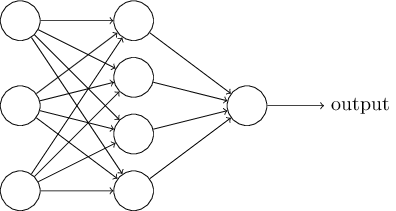
\includegraphics[scale=0.5]{images/neuron}
	\caption{A model of neural networks}
	\label{fignnnetworks}
\end{figure}
The image \ref{fignnnetworks} shows a simple model of neural networks. The leftmost layer in this network is called the input layer, the rightmost layer is called the output layer. The neurons within the input layer are called input neurons, the neurons from output layer are called output neurons. When design the network, the input and the output are often straightforward. It means that the neural networks is designed where the output from one layer is used as the input to the next layer, there are no loops in the network, it always feed forward, never feed back, called feedforward networks. The size of a neural network can be to compute as the number of neurons, or the number of parameters.

\section{Deep network}
A deep neural network is a neural network with multiple layers between the input and the output layers. These layers are called hidden layers. Each layer tries to find the correct mathematical operator to turn its input into the next layer. At each layer excepts the output layer, the output is indicated by an activation function i.e sigmoid, tanh, \ldots before transfer to the next layer. Fig. \ref{fignnnetworks} shows an deep network example with one hidden layer. The deep neural network forwards the data from the input layer to the output layer without looping back: The network creates the connections of neurons and assigns the ``weight" for each connection. At each layer, the weights and its input are multiplied and return an output. Further, an algorithm is used to adjust the weights so that make certain parameters more influential until it receives the correct mathematical manipulation on all dataset.

Besides the deep neural network, Convolutional Neural Networks are other solutions for deep learning. It is also similar to neural network. It also consists of an input, an output, as well as multiple hidden layers. The hidden layers of a CNN may be convolutional layers, pooling layers, normalization layers or fully connected layers. An only difference is CNN receives the structured data as the input i.e. images. This change makes the forward functions more efficient and vastly reduce the number of parameters in the network because some of layers in CNN do not contain the learnable parameters i.e. pooling layer or dropout layer. The layers of a CNN has neurons arranged in three dimensions of the input: \textit{width, height and depth} with learnable parameters.

\section{Convolutional neural network}
A Convolutional Neural Network (CNN) is made from a sequential of layers. It takes images as an input, then the images are passed through the series of layers and get the result at the output layer. At each layer, a different function is applied to transform the input data depending on the type of layer. The common layers are used to desgin the CNN includes: convolutional layer, pooling layer, dropout layer, full-connected layer, \ldots. Fig. \ref{} shows an example of a CNN. The image is passed through the functions (i.e. convolution, subsampling) corresponding to the layers of the network before proceduing the output.

\begin{figure}[h]
	\centering
	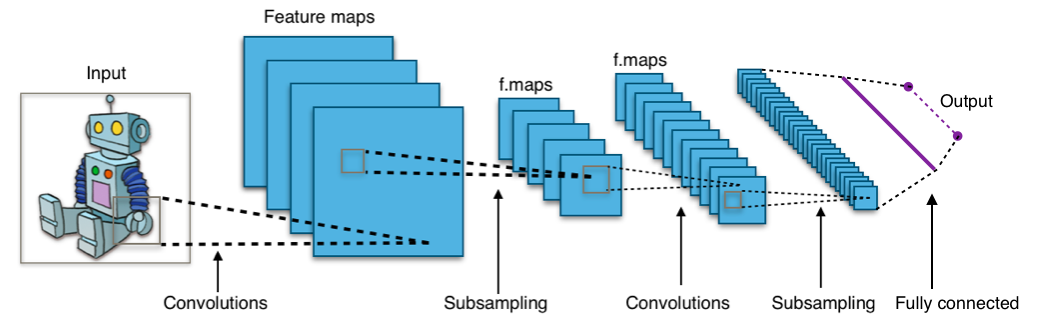
\includegraphics[scale=0.45]{images/cnn_architecture}
	\caption{An architecture of convolutional neural network}
	\label{figlncex}
\end{figure}~\\

In a CNN network, each layer is corresponding to a kind of mathematic computing, i.e convolution, down-sampling or dropping, \ldots to effect on the input and to produce the output. Depending on the type of computing, it can be required the learnable parameters or not. In this part, we will discribe the characteristics of the popular layers in a CNN.
\subsection{Convolutional layer}
Convolutional layer (CONV) is the most popular layer in CNN. CONV layer uses a set of learnable filters as parameters. Each filter is a small spatially but extends the depth of the input. During the computing process, the filters are slided over each pixel of the input (from left to right, top to bottom) to compute dot product between its the entries and the input at this position. For each filter, the response at the output may be the orientation of the edges or a blotch of color. With an entire set of filters in CONV layer, the outputs will be stacked along the depth dimension.

In neural network, a neuron of a layer is connected to all neurons of the next layer, it makes the learnable parameters of a neural network become large. In the case of CONV layer is different, it connects each neurons to only a local region of the input. The spatial extent of the connectivity is a hyperparameter called the receptive field of the neuron (equals to the number of filters). The extent of connectivity has the depth axis equal to the depth of the input. For example, if the input has the size of $[32 \times 32 \time 3]$ and the filter has size of $[5 \time 5]$, then each neuron in CONV layer will heave the weights to a $[5 \time 5 \times 3]$ region in the input (it means we will have $5 * 5 * 3  = 75$ weights. So, with 3 hyperparameters of a CONV layer (depth, stride and zero-padding), we can control the size of its output as equation following: 

\begin{equation}
	N = \frac{(W - F + 2P)}{S} + 1
	\label{convneuron}
\end{equation}
Where:
\begin{itemize}
	\item \textbf{W} is the input size
	\item \textbf{F} is the filter size of CONV layer neurons
	\item \textbf{P} is amount of zero padding on the border
	\item \textbf{S} is the stride.
\end{itemize}

In three hyperparameters of CONV layer: the \textbf{depth} parameters corresponds to the number of the filters; the \textbf{stride} parameter describes how many pixels we slide the filter in each time; the \textbf{zero-padding} parameter uses when we would like to pad the input with zeros around the border, the important parameter is stride. If we choose the stride inadequate, the result could be not integer, it means that the neurons do not fit neatly and symmetrically across the input. Besides, using zero-padding also affects to the spatial size of the output.

\subsection{Pooling layer}

\section{CNN Frameworks}
